\documentclass[epsfig,10pt,fullpage]{article} \addtolength{\textwidth}{1.5in}
\addtolength{\oddsidemargin}{-0.75in}
\addtolength{\topmargin}{-0.75in}
\addtolength{\textheight}{1.5in}
\addtolength{\evensidemargin}{0.75in}
\raggedbottom
\usepackage{ae,aecompl}
\usepackage{epsfig,float,times}
\usepackage{graphicx}
\usepackage[usenames]{xcolor}

\newcommand{\red}[1]{{\color{red}\sf{#1}}}
\newcommand{\blue}[1]{{\color{blue}\sf{#1}}}

\usepackage{placeins}
\usepackage{listings}
\definecolor{PineGreen}{rgb}{0.0, 0.47, 0.44}
\definecolor{ForestGreen}{rgb}{0.13, 0.55, 0.13}
\definecolor{Brown}{rgb}{0.59, 0.29, 0.0}

\lstdefinelanguage{ASM}{
  morekeywords = [1]{mv, mvt, add, sub, st, ld, and, b, bne, beq, bcc, bcs, bpl, bmi},
  morekeywords = [2]{word, define},
  keywordstyle = [1]\color{ForestGreen},
  keywordstyle = [2]\color{blue},
  sensitive = true,
  morecomment = [l]{//},
}
\lstset{
%language = C,
%language = Verilog,
language = ASM,
basicstyle=\small\color{black}\ttfamily, commentstyle=\small\color{Brown}\itshape\ttfamily,
showstringspaces=false,
frame=none, %lines % boxed listings
breaklines=true,
breakatwhitespace=true,
tabsize=3
}
\setcounter{table}{2}
\setcounter{figure}{11}

\begin{document}
~\\
\centerline{\huge Laboratory Exercise 10}
~\\
\centerline{\large An Enhanced Processor}
~\\
In Laboratory Exercise 9 we described a simple processor. In
Part I of that exercise the processor itself was designed, and in Part II the processor was
connected to an external counter and a memory unit. This exercise describes subsequent
parts of the processor design. The numbering of figures and tables in this exercise 
are continued from those in Parts I and II of the preceding lab exercise.

~\\
\noindent
In this exercise we will extend the capability of the processor so that the external counter 
is no longer needed, and so that the processor can perform read and
write operations using memory or other devices. 
A schematic of the enhanced processor is given in
Figure~\ref{fig:fig12}. In this figure
registers $r0$ to $r6$ are the same as in Figure~1 of Lab~9, but register $r7$ has 
been changed to a counter. This counter is used to provide the addresses in the memory from 
which the processor's instructions are read; in the preceding 
lab exercise, a counter external to the processor was used for this purpose. 
We will refer to $r7$ as the processor's {\it program counter} ({\it pc}), because this 
terminology is common for real processors available in the industry. When the processor is 
reset, {\it pc} is set to address 0. At the start of each instruction (in time step $T_0$) the 
value of {\it pc} is used as an address to read an instruction from the memory. The instruction
returned from the memory is stored into the {\it IR} register and the {\it pc} is automatically
incremented to point to the next instruction.

~\\
\noindent
The processor's control unit increments {\it pc} by using the {\it pc\_incr} signal, which is
just an enable on this counter. It is also possible to load an arbitrary address into 
{\it pc} by having the processor execute an instruction in which the destination register is 
specified as {\it pc}. In this case the control unit uses
{\it pc}$_{in}$ to perform 
a {\it load} of the counter. Thus, the processor can execute instructions at any address 
in the memory, as opposed to only being able to execute instructions that are stored at 
successive addresses. The current contents of {\it pc},
which always has the address of 
the {\it next} instruction to be executed, can be copied into another register if needed 
by using a {\it mv} instruction. 

~\\
\noindent
The enhanced processor will have four new instructions, which are listed
in Table~\ref{tab:new_instr}.  The {\it ld} (load) instruction {\it reads} data into 
register {\it rX} from the external memory address specified in register {\it rY}. Thus, 
the syntax [{\it rY}] means that the contents of register {\it rY} are used as an
{\it external address}. The {\it st} (store) instruction {\it writes} the data contained 
in register {\it rX} into the memory address found in {\it rY}. The {\it and} instruction 
is similar to the {\it add} and {\it sub} instructions that were introduced in Lab 9.
This instruction extends the adder/subtracter unit in the processor into an
{\it arithmetic logic unit}. Besides performing addition and subtraction, it 
has the ability to generate a bit-wise logical AND (\&) of the destination register
{\it rX} with the second operand {\it Op2}. As discussed
in Lab 9, the operand {\it Op2} can be either another register {\it rY}, or immediate
data {\it \#D}.

~\\
\noindent
The {\it b\{cond\}} instruction in Table~\ref{tab:new_instr} is used 
to cause a processor {\it branch}, which means to
change the program counter ({\it pc}) to the address of a specific instruction. The {\it cond}
part of the branch instruction is optional and represents a {\it condition}. The instruction 
loads the address {\it Label} into {\it pc} only if the specified condition evaluates to true.
An example of a condition is {\it eq}, which stands for {\it equal} (to zero). 
The instruction \texttt{beq Label} will load the address {\it Label} into {\it pc} if the
last result produced by the arithmetic logic unit, which is stored in register $G$, was 0. 
The 3-bit register $F$ shown in Figure~\ref{fig:fig12} is required for the {\it b\{cond\}} 
instruction, which is discussed in more detail in Part V.

\begin{table}[H]
\begin{center}
\begin{tabular}{l|c}
\rule[-0.075in]{0in}{0.25in}Operation & Function performed \\ \hline 
\rule[-0.075in]{0in}{0.25in}{\it ld}~~~{\it rX}, [{\it rY}] & {\it rX} $\leftarrow$ [{\it rY}] \\ 
\rule[-0.075in]{0in}{0.25in}{\it st}~~~{\it rX}, [{\it rY}] & [{\it rY}] $\leftarrow$ {\it rX} \\ 
\rule[-0.075in]{0in}{0.25in}{\it and}~~~{\it rX}, {\it Op2} & {\it rX} $\leftarrow$ {\it rX} \& {\it Op2} \\ 
\rule[-0.075in]{0in}{0.25in}{\it b\{cond\}}~~~{\it Label} & if ({\it cond}), {\it pc} $\leftarrow$ {\it Label} \\ 
\end{tabular}
\caption{New instructions in the enhanced processor.}
\label{tab:new_instr}
\end{center}
\end{table}

\begin{figure}[H]
\begin{center}
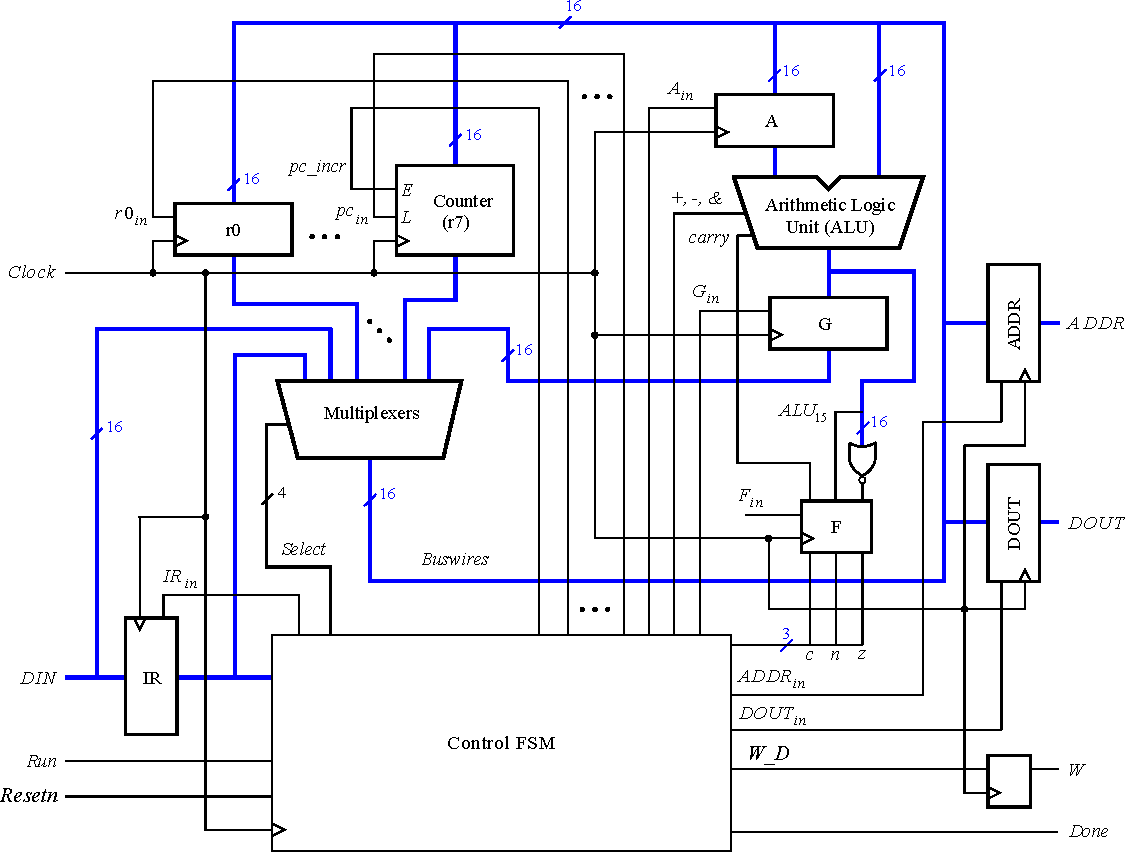
\includegraphics[scale = 0.8]{figures/figure12_F.pdf}
\end{center}
\caption{An enhanced version of the processor.}
\label{fig:fig12}
\end{figure}

~\\
\noindent
Recall from Lab 9 that instructions are encoded using a 16-bit format. For instructions
that specify {\it Op2} as a register the encoding is \texttt{III0XXX000000YYY}, and if {\it Op2}
is an immediate constant the format is \texttt{III1XXXDDDDDDDDD}. You should use these 
same encodings for this exercise. Assume that \texttt{III} $= 100$ for the {\it ld} instruction,
$101$ for {\it st}, and $110$ for {\it and}. The encoding for {\it b\{cond\}} is discussed 
in Part V of this exercise.

~\\
Figure~\ref{fig:fig12} shows two registers in the processor that are used for data transfers. The 
{\it ADDR} register is used to send addresses to an external device, such as a memory module,
and the {\it DOUT} register is used by the processor to provide data that is to be stored outside 
of the processor. One use of the {\it ADDR} register is for reading, or {\it fetching}, 
instructions from memory; when the processor wants to fetch an instruction, the contents
of {\it pc} are transferred across the bus and loaded into {\it ADDR}. This address is 
provided to the memory.

~\\
In addition to fetching instructions, the processor can read data 
at any address by using the {\it ADDR} register. Both data and instructions are read into 
the processor on the {\it DIN} input port.  The processor can write data for storage at 
an external address by placing this address into the {\it ADDR} register, placing the data 
to be stored into the {\it DOUT} register, and asserting the output of the {\it W} 
({\it Write}) flip-flop to 1. 

\section*{Connecting the Processor to External Devices}

Figure~\ref{fig:fig13} illustrates how the enhanced processor can be connected to memory and 
other devices. The memory unit in the figure is 16-bits wide and 256-words deep.  A diagram 
of this memory is given in Figure~\ref{fig:fig14}.
It supports both read and write operations and therefore has both address and 
data inputs, as well as a write-enable input. As depicted in Figure~\ref{fig:fig14},
the memory has a clock input that is used to store the address, data, and write enable 
inputs into registers.  This type of memory unit is called a {\it synchronous}
static random access memory (SSRAM). 

~\\
Figure~\ref{fig:fig13} also includes a 9-bit output port (register) that can be used to store 
data from the processor. In the figure this output port is connected to a set of LEDs, like 
those available on the DE1-SoC, and similar, FPGA boards. To allow the processor to select 
either the memory 
unit or output port when performing a write operation, the circuit includes {\it address decoding},
which is done using NOR gates and AND gates. Let the processor's address lines be referred
to as ADDR = $A_{15} A_{14} \cdots A_1 A_0$. 
If the upper address lines $A_{15} A_{14} A_{13} A_{12} = 0000$, then the memory unit 
can be written. Figure~\ref{fig:fig13} shows $n$ {\it lower} address lines connected from the 
processor to the memory; since the memory has 256 words, then $n = 8$ and the memory's 
{\it address} port is driven by the processor address lines $A_7 \ldots A_0$. For
addresses in which $A_{15} A_{14} A_{13} A_{12} = 0001$, the data written by the processor
is loaded into the output port connected to {\it LEDs} in Figure~\ref{fig:fig13}.
~\\
\begin{figure}[H]
\begin{center}
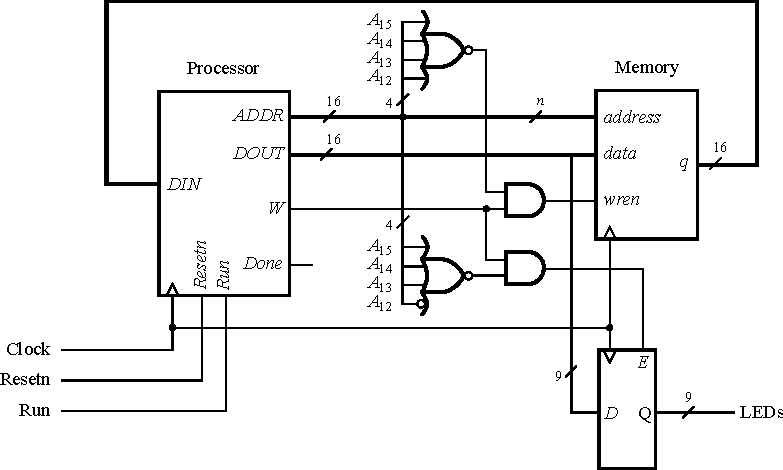
\includegraphics{figures/figure13.pdf}
\end{center}
\vspace{-0.5cm}
\caption{Connecting the enhanced processor to a memory unit and output register.}
\label{fig:fig13}
\end{figure}

\begin{figure}[b]
\begin{center}
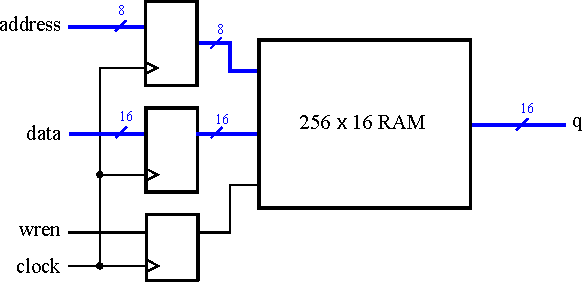
\includegraphics{figures/figure14.pdf}
\end{center}
\vspace{-0.5cm}
\caption{The synchronous SRAM unit.}
\label{fig:fig14}
\end{figure}

\section*{Part III}

Figure~\ref{fig:top} gives Verilog code for a top-level file that you can use for this
part of the exercise. The input and output ports for this module are chosen so that it can
be implemented on a DE1-SoC, or similar, board. The Verilog code corresponds to the circuit 
in Figure~\ref{fig:fig13},
plus an additional input port that is connected to switches {\it SW}$_8$ $\ldots$ {\it SW}$_0$.
This input port can be read by the processor at addresses in which $A_{15} \ldots A_{12} = 0011$.
(Switch {\it SW}$_9$ is not a part of the input port, because it is dedicated for use as the
processor's {\it Run} input.) To support reading from both the SW input port and the memory
unit, the top-level circuit includes a multiplexer that feeds the processor's {\it DIN}
input. This multiplexer is described by using an \texttt{if-else} statement inside 
the \texttt{always} block in Figure~\ref{fig:top}.

~\\
\noindent
The code in Figure~\ref{fig:top} is provided with this exercise, along with a few
other source-code files: {\it flipflop.v}, {\it inst\_mem.v}, {\it inst\_mem.mif}, and 
(part of) {\it proc.v}. The {\it inst\_mem.v} source-code file was created by using the Quartus IP 
Catalog to instantiate a \texttt{RAM:1-PORT} memory module. It has a 16-bit wide read/write
data port and is 256-words deep, corresponding to Figure~\ref{fig:fig14}.

~\\
\noindent
The Verilog code in the {\it proc.v} file implements register {\it r7} as a program counter,
as discussed above, and includes a number of changes that are needed to support the 
new {\it ld}, {\it st}, {\it and}, and {\it b\{cond\}} instructions. In this part you are to 
augment this Verilog code to complete the implementation of the {\it ld} and
{\it st} instructions, as well as the {\it and} instruction. You do not 
need to work on the {\it b\{cond\}} instruction for this part. 

\lstset{language=Verilog,numbers=none,escapechar=|}
\begin{figure}[h]
\begin{center}
\begin{minipage}[h]{15 cm}
\begin{lstlisting}[name=proc]
|\label{line:module}|module part3 (KEY, SW, CLOCK_50, LEDR);
	input [0:0] KEY;
	input [9:0] SW;
	input CLOCK_50;
	output [9:0] LEDR;	

	wire [15:0] DOUT, ADDR;
	wire Done, W;
	reg [15:0] DIN;
	wire inst_mem_cs, SW_cs, LED_reg_cs;
	wire [15:0] inst_mem_q;
	wire [8:0] LED_reg, SW_reg;      // LED[9] and SW[9] are used for Run

   proc U3 (DIN, KEY[0], CLOCK_50, SW[9], DOUT, ADDR, W, Done);

	assign inst_mem_cs = (ADDR[15:12] == 4'h0);
	assign LED_reg_cs = (ADDR[15:12] == 4'h1);
	assign SW_cs = (ADDR[15:12] == 4'h3);
	inst_mem U4 (ADDR[7:0], CLOCK_50, DOUT, inst_mem_cs & W, inst_mem_q);

	always @ (*)                     // input multiplexer
	   if (inst_mem_cs == 1'b1)
		   DIN = inst_mem_q;
	   else if (SW_cs == 1'b1)
		   DIN = {7'b0000000, SW_reg};
	   else
		   DIN = 16'bxxxxxxxxxxxxxxxx;

	regn #(.n(9)) U5 (DOUT[8:0], Resetn, LED_reg_cs & W, CLOCK_50, LED_reg);
	assign LEDR[8:0] = LED_reg;
   assign LEDR[9] = SW[9];

	regn #(.n(9)) U7 (SW[8:0], Resetn, 1'b1, CLOCK_50, SW_reg); // Run = SW[9]
endmodule
\end{lstlisting}
\end{minipage}
\caption{Verilog code for the top-level file.}
\label{fig:top}
\end{center}
\end{figure}

\newpage
\noindent
Perform the following:
\begin{enumerate}
\item Augment the code provided in {\it proc.v} so that the enhanced processor reads each
of its instructions from the external memory, using the program counter to provide the
memory address. Also, implement the {\it ld}, {\it st}, and {\it and} instructions. The
control FSM requires six time steps for the enhanced processor, as indicated in 
Table~\ref{tab:control_signals}.  The first three steps are needed to {\it fetch} 
an instruction into the processor from memory. In step $T_0$ 
the program counter is copied into the {\it ADDR} register, so that this
address will be provided to the memory. This action is accomplished by placing the program
counter onto the {\it Buswires}, and asserting {\it ADDR}$_{in}$. Also, 
{\it pc\_incr} is asserted so that the program counter will be incremented
to the address in memory of the next instruction. Since the memory has a synchronous
interface, as shown in Figure~\ref{fig:fig14}, the processor must use time-step $T_1$ to 
wait for the memory to respond. Then, the {\it IR$_{in}$} signal can be asserted in step
$T_2$, so that in step $T_3$ the {\it IR} register will hold the machine code of the
instruction to be executed. 

We can compare the time steps in the enhanced processor to those of the simple processor from
Laboratory Exercise~9. In the enhanced processor, step $T_2$ serves the same function as 
step $T_0$ in the simple processor. Thus, in Table~\ref{tab:control_signals} the control signals
asserted in steps $T_2$ to $T_5$ for the {\it mv}, {\it mvt}, {\it add}, and {\it sub} 
instructions are the same as those used in time steps $T_0$ to $T_3$ for the simple processor. 
The {\it and} instruction uses the same control signals as for {\it add} and {\it sub},
with one difference---for {\it and}, the control signal {\it ALU\_and} is asserted in 
step $T_4$, which causes the ALU to perform the logical AND operation.

The last two lines in Table~\ref{tab:control_signals} show the timing needed for {\it ld}
and {\it st}. In both instructions the contents of register {\it rY} is
transferred in step $T_3$ to the {\it ADDR} register. For {\it ld} the processor uses 
$T_4$ to wait for the memory to respond with data, and then step
$T_5$ causes this data to
be loaded into register {\it rX}. For {\it st}, the data in
{\it rX} to be written to the
memory is transferred to register {\it DOUT} in step $T_4$, and {\it W\_D} (see 
Figure~\ref{fig:fig12}) is asserted to set the {\it W} ({\it write}) signal for the memory.  

\begin{table}[H]
\begin{center}
\begin{tabular}{r|c|c|c|c|c|c|}
\multicolumn{1}{c}{~} & \multicolumn{1}{c}{$T_0$} & \multicolumn{1}{c}{$T_1$} & \multicolumn{1}{c}{$T_2$} & \multicolumn{1}{c}{$T_3$} & \multicolumn{1}{c}{$T_4$} & \multicolumn{1}{c}{$T_5$} \rule[-0.075in]{0in}{0.25in}\\ \cline{2-7}
{\it mv~} & {\it Select} {\it pc}, & ~ & {\it IR}$_{in}$ & \rule[-0.075in]{0in}{0.25in}{\it Select} {\it rY} or {\it IR}, &  &  \\
~ & {\it ADDR}$_{in}$, {\it pc\_incr} & ~ & ~ & {\it rX$_{in}$}, {\it Done} &  &  \\ \cline{2-7}
{\it mvt~} & {\it Select} {\it pc}, & ~ & {\it IR}$_{in}$ & \rule[-0.075in]{0in}{0.25in}{\it Select} {\it IR}, &  &  \\
~ & {\it ADDR}$_{in}$, {\it pc\_incr} & ~ & ~ & {\it rX$_{in}$}, {\it Done} &  &  \\ \cline{2-7}
\rule[-0.075in]{0in}{0.25in}{\it add~} & {\it Select} {\it
pc}, & ~ & {\it IR}$_{in}$ & {\it Select} {\it rX}, & {\it Select} {\it rY} or {\it IR}, & {\it Select G}, {\it rX$_{in}$}, \\
~ & {\it ADDR}$_{in}$, {\it pc\_incr} & ~ & ~ & {\it A$_{in}$} &  {\it G$_{in}$} & {\it Done} \\
\cline{2-7}
\rule[-0.075in]{0in}{0.25in}{\it sub~} & {\it Select} {\it
pc}, & ~ & {\it IR}$_{in}$ & {\it Select} {\it rX}, & {\it Select} {\it rY} or {\it IR}, & {\it Select G}, {\it rX$_{in}$}, \\
~ & {\it ADDR}$_{in}$, {\it pc\_incr} & ~ & ~ & {\it A$_{in}$} &  {\it AddSub}, {\it G$_{in}$} & {\it Done} \\
\cline{2-7}
\rule[-0.075in]{0in}{0.25in}{\it and~} & {\it Select} {\it
pc}, & ~ & {\it IR}$_{in}$ & {\it Select} {\it rX}, & {\it Select} {\it rY} or {\it IR}, & {\it Select G}, {\it rX$_{in}$}, \\
~ & {\it ADDR}$_{in}$, {\it pc\_incr} & ~ & ~ & {\it A$_{in}$} &  {\it ALU\_and}, {\it G$_{in}$} & {\it Done} \\
\cline{2-7}
\rule[-0.075in]{0in}{0.25in}{\it ld~} & {\it Select} {\it
pc}, & ~ & {\it IR}$_{in}$ & {\it
Select} {\it rY}, &  & {\it Select DIN}, {\it rX$_{in}$}, \\
~ & {\it ADDR}$_{in}$, {\it pc\_incr} & ~ & ~ & {\it ADDR}$_{in}$ &  & {\it Done} \\
\cline{2-7}
\rule[-0.075in]{0in}{0.25in}{\it st~} & {\it Select} {\it
pc}, & ~ & {\it IR}$_{in}$ & {\it
Select} {\it rY}, & {\it Select rX}, {\it DOUT$_{in}$}, & \\
~ & {\it ADDR}$_{in}$, {\it pc\_incr} & ~ & ~ & {\it ADDR$_{in}$} & $W_D$, {\it Done} & \\
\cline{2-7}
\end{tabular}
\caption{Control signals asserted in each instruction/time step.}
\label{tab:control_signals}
\end{center}
\end{table}

Test your Verilog code by using the Questa or ModelSim
Simulator. Sample setup files for the Simulator, including a testbench, are provided along with 
the other design files for this exercise.  The sample testbench first resets the processor system
and then asserts the {\it Run} switch, {\it SW}$_9$, to 1. A sample program to test your 
processor is also provided, in a file called {\it inst\_mem.mif}. This file represents the 
assembly-language program shown in Figure~\ref{fig:assembly}, which tests 
the {\it ld} and {\it st} instructions by reading the values of the SW switches and writing 
these values to the LEDs, in an endless loop. At the beginning of a simulation, the Simulator 
loads the contents of the file {\it inst\_mem.mif} into the {\it inst\_mem} memory module, so
that the program can be executed by the processor.  Examine the signals inside 
your processor, as well as the external LEDR values, as the program executes within the
simulation.

An {\it Assembler} software tool, called {\it sbasm.py}, is provided for use with your processor.
The Assembler is written in Python and is included along with the design files for this exercise.
To use this Python script you need to have Python (version 3) installed on your computer. 
The Assembler includes
a README file that explains how to install and use it. The {\it sbasm.py} Assembler can 
generate machine code for all of the processor's instructions. The provided file 
{\it inst\_mem.mif} was created by using {\it sbasm.py} to {\it assemble} the program in 
Figure~\ref{fig:assembly}. As the figure indicates, you can define symbolic
constants in your code by using the .\blue{define} {\it directive}, and you can use 
labels to refers to lines of code, such as \texttt{MAIN}.
Comments are specified in the code by using \texttt{//}. The Assembler ignores anything 
on a line following \texttt{//}.

\lstset{language=ASM,numbers=none,escapechar=|}
\begin{figure}[H]
\begin{center}
\begin{minipage}[h]{12.5 cm}
\begin{lstlisting}[name=proc]
|\label{line:module}|.define LED_ADDRESS 0x10
.define SW_ADDRESS 0x30

// Read SW switches and display on LEDs
			mvt	r3, #LED_ADDRESS	// point to LED port
			mvt	r4, #SW_ADDRESS	// point to SW port
MAIN:		ld		r0, [r4]				// read SW values
			st		r0, [r3]				// light up LEDs
			mv 	pc, #MAIN
\end{lstlisting}
\end{minipage}
\caption{Assembly-language program that uses {\it ld} and {\it st} instructions.}
\label{fig:assembly}
\end{center}
\end{figure}

An example simulation result for a correctly-designed circuit 
is given in Figure~\ref{fig:part3}. It shows the execution of the first four instructions
in Figure~\ref{fig:assembly}.

\item Once your simulation results look correct, you can then implement your Verilog
code on an FPGA board, such as the DE1-SoC. However, as we mentioned in Lab Exercise~9, as
an interim step you may wish to first simulate your processor by using the graphical user
interface (GUI) provided by the DESim tool---it gives a convenient way of observing the behaviour 
of programs running on your processor that use the lights, switches, and other features of 
the board. You are encouraged to make use of DESim, as it
is a convenient way of debugging issues, especially when you do not have access to a 
physical board.

The setup files that are needed to use DESim for this part of the exercise are provided along
with its design files.  When using DESim, the memory module in your design will be initialized with
the contents of the {\it inst\_mem.mif} file, so that the program in the memory 
can be executed by your processor. Once you start the simulation within the DESim GUI make sure to 
reset the circuit by clicking on the \texttt{Push Button} that corresponds to
\texttt{KEY}$_0$, and assert the {\it Run} signal to 1 by setting the \texttt{Switch}
that corresponds to \texttt{SW}$_9$. Toggle the values of the \texttt{Switches}
\texttt{SW}$_{8-0}$ in the DESim GUI and observe the \texttt{LEDs}. 

\item
To implement your Verilog code using an actual (as opposed to {\it simulated}, with DESim) 
DE1-SoC board, you have to use the Quartus Prime software.
A sample Quartus project file, {\it part3.qpf}, and Quartus
settings file, {\it part3.qsf}, are provided with the exercise. After compiling your code 
with the Quartus software, generate a .qsf file in and upload it to the NO-IDE lab of LabsLand. Toggle the SW switches and observe the LEDs to test your circuit.
\end{enumerate}

\begin{figure}[H]
	\begin{center}
		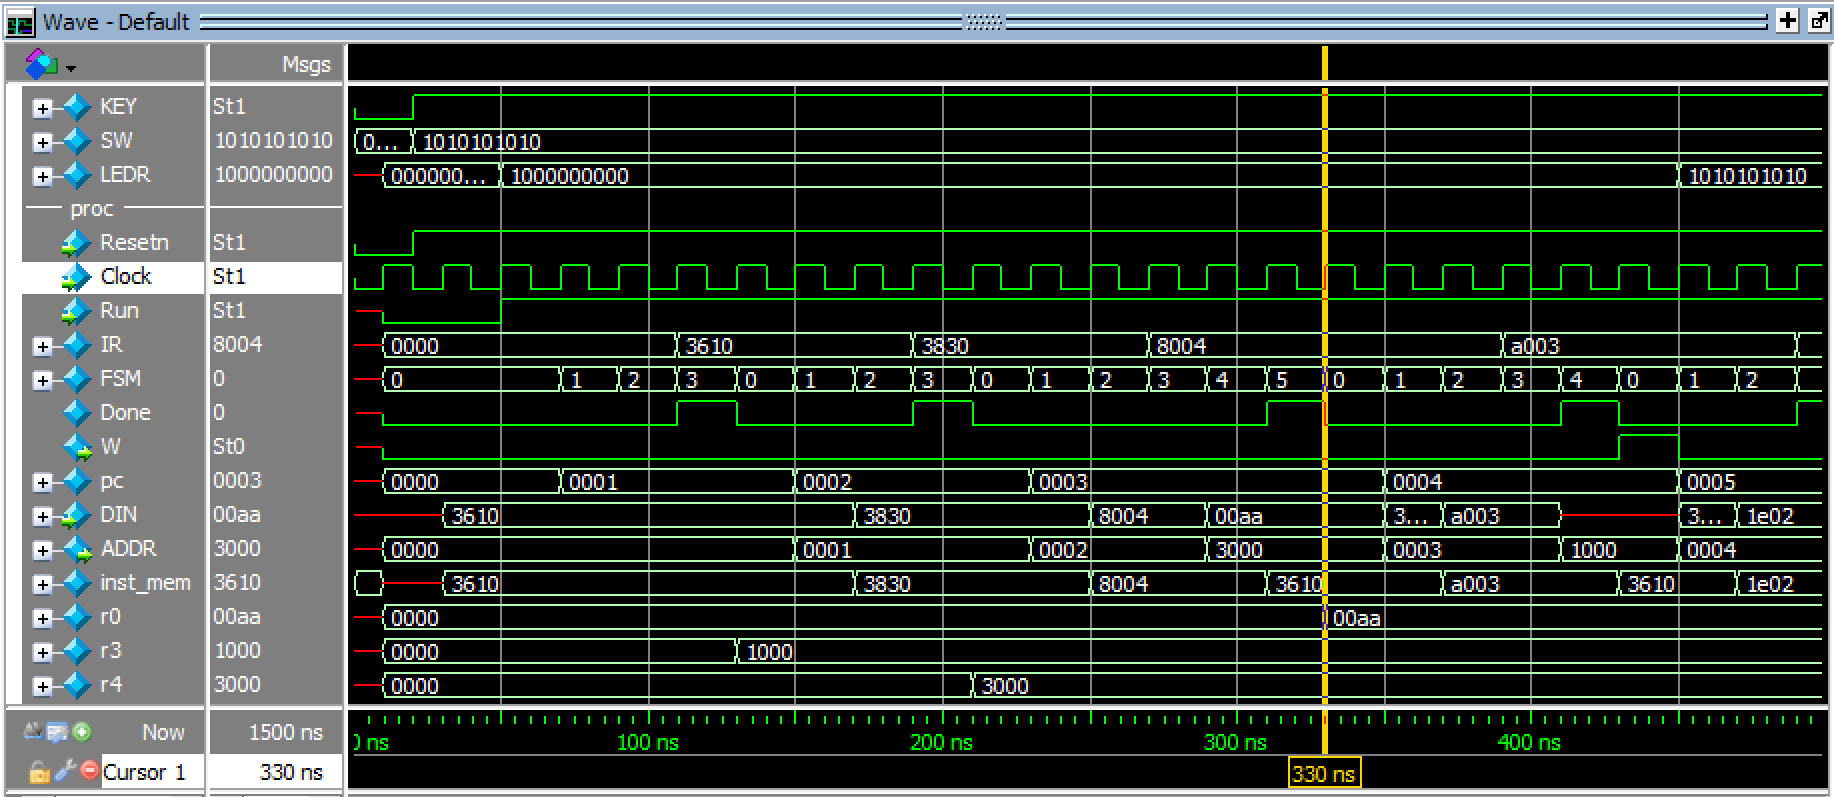
\includegraphics[width=\textwidth]{figures/part3.png}
	\end{center}
	\caption{Simulation results for the processor.}
	\label{fig:part3}
\end{figure}

\section*{Part IV}
In this part you are to create a new Verilog module that represents an output port called 
{\it seg7}. It will allow your processor to write data to each of the six 7-segment
displays that are available on a DE1-SoC, or similar, board. The {\it seg7} module will 
include six write-only seven-bit registers,
one for each display. Each register should directly drive the segment lights for one 
seven-segment display, so that the processor can write characters onto the displays. 

~\\
\noindent
Perform the following:

\begin{enumerate}
\item A top-level file is provided for this part
called {\it part4.v}. The top-level module has output ports for connecting
to each of the 7-segment displays. 
For each display, segment 0 is on the top of the display, and then segments 1 to 5 are assigned
in a clockwise fashion, with segment 6 being in the middle of the display.

The {\it part4.v} Verilog code includes address decoding for the new {\it seg7} module, 
so that processor addresses in which $A_{15} A_{14} A_{13} A_{12} = 0010$ select this module.
The intent is that address \texttt{0x2000} should write to the register that controls 
display {\it HEX0}, \texttt{0x2001} should select the register for {\it HEX1}, and 
so on. For example, if your processor 
writes \texttt{0} to address \texttt{0x2000}, then the {\it seg7} module
should turn off all of the segment-lights in the {\it HEX0} display; writing \texttt{0x7f} 
should turn on all of the lights in this display. 

\item 
You are to complete the partially-written Verilog code in the file {\it seg7.v}, so that
it contains the required six registers---one for each 7-segment display. 
        
\item You can compile and test your Verilog code by using the Simulator setup files that 
are provided for this part of the exercise. An {\it inst\_mem.mif} file is also provided
that corresponds to the assembly-language program shown in 
Figure~\ref{fig:7segs}. This program works as follows: it reads the {\it SW} switch port and 
lights up a seven-segment display corresponding to the value read on {\it SW}$_{2-0}$. For
example, if {\it SW}$_{2-0} = 000$, then the digit~\texttt{\red{0}} is shown on {\it HEX0}.
If {\it SW}$_{2-0} = 001$, then the digit~\texttt{\red{1}} is displayed on {\it HEX1}, 
and so on, up to the digit~\texttt{\red{5}} which would be shown on {\it HEX5} if
{\it SW}$_{2-0} = 101$.

\item Once your simulation results look correct, you can then implement your Verilog
code on an FPGA board. As we discussed in Part III, above, you are encouraged 
to make use of the DESim tool for testing your processor and
programs (project set-up files for DESim are included with this exercise). 
When using your processor, remember to reset the circuit and set {\it Run} $= 1$, and then 
toggle the values of the \texttt{Switches} and 
observe the \texttt{Seven-segment Displays}. When compiling your Verilog code with
Quartus Prime, you may wish to make use of the sample Quartus project file, {\it part4.qpf}, 
and Quartus settings file, {\it part4.qsf}, that are included along with this exercise.
\end{enumerate}

\lstset{language=ASM,numbers=none,escapechar=|}
\begin{figure}[H]
\begin{center}
\begin{minipage}[h]{15 cm}
\begin{lstlisting}[name=proc]
|\label{line:module}|
.define HEX_ADDRESS 0x20
.define SW_ADDRESS 0x30

// This program shows the digits 543210 on the HEX displays. Each digit has to
// be selected by using the SW switches.
MAIN:   mvt    r2, #HEX_ADDRESS     // point to HEX port
        mv     r3, #DATA            // used to get 7-segment display pattern

        mvt    r4, #SW_ADDRESS      // point to SW port
        ld     r0, [r4]             // read switches
        and    r0, #0x7             // use only SW2-0
        add    r2, r0               // point to correct HEX display
        add    r3, r0               // point to correct 7-segment pattern

        ld     r0, [r3]             // load the 7-segment pattern
        st     r0, [r2]             // light up HEX display

        mv     pc, #MAIN

DATA:   .word  0b00111111           // '0'
        .word  0b00000110           // '1'
        .word  0b01011011           // '2'
        .word  0b01001111           // '3'
        .word  0b01100110           // '4'
        .word  0b01101101           // '5'
\end{lstlisting}
\end{minipage}
\caption{Assembly-language program that tests the seven-segment displays.}
\label{fig:7segs}
\end{center}
\end{figure}

\section*{Part V}
In this part you are to enhance your processor so that it implements the {\it b\{cond\}}
instruction.  The {\it conditions} supported by the processor are called 
{\it eq}, {\it ne}, {\it cc}, {\it cs}, {\it pl}, and {\it mi}, which means that the variations 
of the branch instruction are {\it b}, {\it beq}, {\it bne}, {\it bcc}, and so on. The {\it b}
instruction {\it always} branches. For example, \texttt{b  MAIN} loads the address of the
label \texttt{MAIN} into the program counter. The meanings of the conditional versions are 
explained below.

~\\
\noindent
The instruction \texttt{beq  LABEL} means {\it branch if equal} (to zero). It performs a branch 
(sets {\it pc} $=$ \texttt{LABEL}) if the most recent result of an instruction 
executed using the arithmetic logic unit (ALU), which is stored in register $G$, was~0. 
Similarly, {\it bne} means {\it branch if not
equal} (to zero).  It performs a branch only if the contents of $G$ are not equal to 0.
The instruction {\it bcc} stands for {\it branch if carry clear}. It branches if the last
add/subtract operation did {\it not} produce a carry-out. The opposite branch condition, 
{\it bcs}, {\it branch if carry set}, branches if the most recent add/sub generated a 
carry-out. The conditions {\it bpl} and {\it bmi} allow a branch to be taken when the value 
in register {\it G} is a positive or negative (2's complement) value,
respectively. 

~\\
\noindent
To support the conditional branch instructions, you should create three
{\it condition-code flags}, called {\it z}, {\it n}, and {\it c} in your processor. 
The {\it z} flag should have the value 1 when the ALU generates a result of zero; 
otherwise {\it z} should be~0.  The {\it n} flag should be 1 when the ALU generates a 
result that is negative, meaning that the most-significant bit (the {\it sign} bit) of the
result is 1; 
otherwise {\it n} should be set to~0. Finally, the {\it c} flag should reflect the carry-out 
from the ALU; this flag should be 1 when an {\it add} instruction generates a carry-out, or 
when a {\it sub} operation does {\it not} generate a borrow. Figure~\ref{fig:fig12} 
indicates how you can implement the flags as the outputs of a three-bit
register, named $F$. The $z$ flag is controlled by a NOR gate that is 
used to check when the output of the ALU 
is zero, the $n$ flag is connected to the sign-bit from the ALU's output, and a carry-out 
from the ALU drives the $c$ flag. These flags are connected to the FSM controller, which 
should examine the flags in the appropriate clock cycles when executing a {\it b\{cond\}}
instruction.

~\\
\noindent
The branch instructions are encoded similarly to the {\it mvt} instruction introduced
in Lab Exercise~9, which has the format \texttt{III1XXXDDDDDDDDD}, with \texttt{III} $= 001$.
The format of {\it b\{cond\}} is \texttt{III0XXXDDDDDDDDD}, where \texttt{III}~$= 001$,
\texttt{XXX} gives the condition, and \texttt{DDDDDDDDD} specifies an {\it offset}.
The condition \texttt{XXX} is encoded
as {\it none} (always branch) $= 000$, {\it eq}~$= 001$, {\it ne} $= 010$, {\it cc} $= 011$, 
{\it cs} $= 100$, {\it pl} $= 101$, and {\it mi} $= 110$.

~\\
\noindent
The {\it offset} \texttt{DDDDDDDDD} is the 2's-complement value
needed to reach the target \texttt{LABEL} relative to the current contents of the {\it pc}
register.  This offset assumes that the {\it pc} has already been incremented after fetching the 
{\it b\{cond\}} instruction from memory. For example, the instruction \texttt{HERE: b HERE} 
would be encoded as \texttt{0010000111111111}, where the offset is the 2's-complement value -1.

~\\
\noindent
Perform the following:

\begin{enumerate}
\item 
Enhance your processor so that it implements the condition-code flags {\it z}, {\it c}, and
{\it n} and supports the {\it b\{cond\}} instruction. Table~\ref{tab:control_b} indicates the 
control signal timing that can be used for this instruction. Step $T_3$ copies the
contents of the {\it pc} into register $A$, in the ALU. This step also checks whether or 
not the branch should be {\it taken}, based upon the {\it condition}. If the 
{\it condition} is not true, indicated in Table~\ref{tab:control_b} using the syntax 
(!{\it cond}), then the {\it Done} signal is asserted to abort the branch instruction. But if
the {\it condition} is satisfied, then the finite state machine will continue to step $T_4$.
This step places the branch offset, which is in the instruction register ({\it IR}), 
onto the {\it Buswires} so that the ALU can add it to the value of the {\it pc} that was
previously copied into register $A$. Finally, step $T_5$ transfers the computed branch-target 
address to the {\it pc}, so that the branch will be taken. 

\begin{table}[H]
\begin{center}
\begin{tabular}{r|c|c|c|c|c|c|}
\multicolumn{1}{c}{~} & \multicolumn{1}{c}{$T_0$} & \multicolumn{1}{c}{$T_1$} & \multicolumn{1}{c}{$T_2$} & \multicolumn{1}{c}{$T_3$} & \multicolumn{1}{c}{$T_4$} & \multicolumn{1}{c}{$T_5$} \rule[-0.075in]{0in}{0.25in}\\ \cline{2-7}
{\it b\{cond\}~} & {\it Select} {\it pc}, & ~ & {\it IR}$_{in}$ &
\rule[-0.075in]{0in}{0.25in}{\it Select} {\it pc}, {\it A}$_{in}$, & {\it Select} {\it
IR},
& {\it Select} {\it G}, {\it pc}$_{in}$, \\
~ & {\it ADDR}$_{in}$, {\it pc\_incr} & ~ & ~ & if (!{\it cond}) {\it Done} & {\it G}$_{in}$ & {\it Done} \\ \cline{2-7}
\cline{2-7}
\end{tabular}
\caption{Control signals asserted for {\it b\{cond\}} in each time step.}
\label{tab:control_b}
\end{center}
\end{table}

To help with testing and debugging of your processor, setup files for a Simulator are
provided, including a testbench. It simulates your processor instantiated in the top-level file
{\it part5.v}, which is the same as the one from Part IV. 
An example {\it inst\_mem.mif} file is also provided, which corresponds 
to the program in Figure~\ref{fig:branches}. This program is quite short, 
which makes it suitable for visual inspection of the waveforms produced by a Simulator. 
The program uses a sequence of instructions that tests the various conditional branches. 
If the program reaches the line of code labelled \texttt{DEAD}, then at least one 
instruction has not worked properly. 

An example of simulation output for a correctly-working
processor is given in Figure~\ref{fig:part5}. It shows the processor executing instructions
near the start of the code in Figure~\ref{fig:branches}. The instruction that is completed
at simulation time 510 ns is \texttt{sub r0, \#1} (\texttt{0x7001}). As shown in the figure,
this instruction causes the zero flag, {\it z}, to become 1. The next instruction loaded
into {\it IR}, at time 570 ns, is \texttt{bne 0x1} (\texttt{0x25fe}). This instruction
does not take the branch, because $z = 1$. Finally, the instruction loaded at 650~ns is 
\texttt{beq~0x5} (\texttt{0x2201}), which does take the branch. 

\item Once your simulation indicates a correctly-functioning processor,
you can implement it on a DE1-SoC, or similar, board. As discussed above in Parts~III and~IV
you can use the DESim tool as a convenient way of testing and debugging your design 
using a simulation of a board, and you can use Quartus Prime to compile and download your 
circuit to a physical board.  The required project set-up files for both DESim and Quartus are
included along with this exercise.  To test your processor, 
you can use the assembly-language program displayed in Figure~\ref{fig:sitbooboosit}. It 
provides code that tests for the correct operation of instructions supported by the 
enhanced processor.  If all of the tests pass, then
the program shows the word \texttt{\red{PASSEd}} on the
\texttt{Seven-segment Displays}. It also shows 
a binary value on the LEDs that represents the number of successful tests performed. If any test
fails, then the program shows the word \texttt{\red{FAILEd}} on the
\texttt{Seven-segment Displays} and 
places on the \texttt{LEDs} the address in the memory of the instruction that caused the failure.
Assemble the program, which is provided in a file called {\it sitbooboosit.s}, by using 
the {\it sbasm.py} assembler. Store the output produced by {\it sbasm.py} in the file
{\it inst\_mem.mif}.

If you compile your processor system using the DESim tool, it uses the current 
contents of the {\it inst\_mem.mif} file to initialize the memory. When simulating your 
processor make sure to reset it by clicking on the \texttt{Push Button} that corresponds to
\texttt{KEY}$_0$. Then, set the {\it Run} signal to 1 by setting the \texttt{Switch}
that corresponds to \texttt{SW}$_9$. If the {\it sitbooboosit} program displays
\texttt{\red{FAILEd}} on the
\texttt{Seven-segment Displays}, then you can identify the
offending instruction by cross-referencing the LED pattern with the corresponding address
in the file {\it inst\_mem.mif}.

\lstset{language=ASM,numbers=none,escapechar=|}
\begin{figure}[H]
\begin{center}
\begin{minipage}[h]{13.5 cm}
\begin{lstlisting}[name=proc]
MAIN:  mv    r0, #2
LOOP:  sub   r0, #1        // subtract to test bne
       bne   LOOP
       beq   T1            // r0 == 0, test beq
       mv    pc, #DEAD
T1:    mvt   r0, #0xFF
       add   r0, #0xFF     // r0 = 0xFFFF
       bcc   T2            // carry = 0, test bcc
       mv    pc, #DEAD
T2:    add   r0, #1
       bcs   T3            // carry = 1, test bcs
       mv    pc, #DEAD
T3:    bpl   T4
       mv    pc, #DEAD
T4:    add   r0, #-1
       bmi   T5
       mv    pc, #DEAD
T5:    b     MAIN
DEAD:  mv    pc, #DEAD
\end{lstlisting}
\end{minipage}
\caption{Assembly-language program that uses various branches.}
\label{fig:branches}
\end{center}
\end{figure}

\begin{figure}[H]
	\begin{center}
		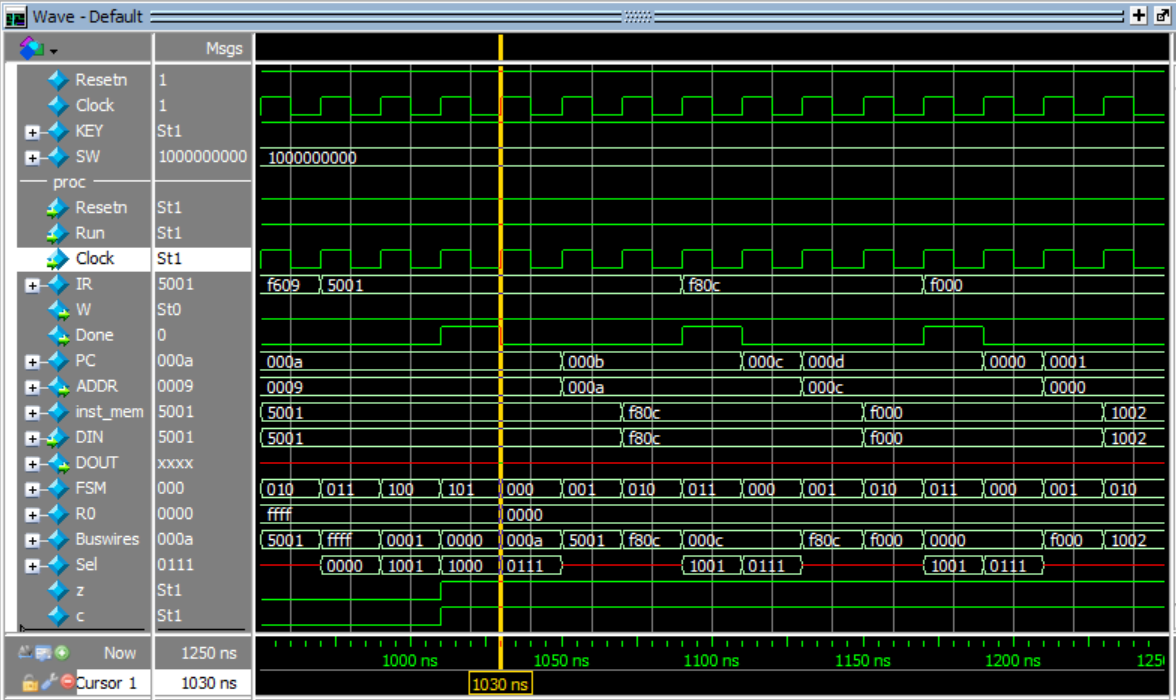
\includegraphics[width=\textwidth]{figures/part5.png}
	\end{center}
	\caption{Simulation results for the processor.}
	\label{fig:part5}
\end{figure}

\begin{figure}[H]
\begin{center}
\begin{minipage}[h]{14 cm}
\begin{lstlisting}[name=proc]
.define LED_ADDRESS 0x10
.define HEX_ADDRESS 0x20

// shows on HEX displays either PASSEd or FAILEd
             mv     r2, #0      // counts each successful test
             mv     r6, #T1     // save address of next test
             sub    r0, r0      // set the z flag
// test bne and beq
T1:          bne    FAIL        // should not take the branch!
             mv     r6, #C1     // save address of next test
C1:          beq    C2          // should take the branch
             mv     pc, #FAIL   // Argh!

C2:          add    r2, #2      // count the last two successful tests
             mv     r6, #T2     // save address of next test
// test bne and beq
T2:          bne    S1          // should take the branch!
             mv     pc, #FAIL
S1:          mv     r6, #C3     // save address of next test
C3:          beq    FAIL        // should not take the branch
             add    r2, #2      // count the last two successful tests
             mv     r6, #T3     // save address of next test
             mv     r3, #-1     // r3 = 0xFFFF
             add    r3, #1      // set the c flag
// test bcc and bcs
T3:          bcc    FAIL        // should not take the branch!
             mv     r6, #C4     // save address of next test
C4:          bcs    C5          // should take the branch
             mv     pc, #FAIL   // Argh!
C5:          add    r2, #2      // count the last two successful tests
             mv     r6, #T4
             mv     r3, #0
             add    r3, r3      // clear carry flag
// test bcc and bcs
T4:          bcc    S2          // should take the branch!
             mv     pc, #FAIL
S2:          mv     r6, #C6     // save address of next test
C6:          bcs    FAIL        // should not take the branch!
             add    r2, #2      // count the last two successes
             mv     r6, #T5     // save address of next test
             mv     r3, #0
             add    r3, #-1
// test bpl and bmi
T5:          bpl    FAIL        // should not take the branch!
             mv     r6, #C7     // save address of next test
C7:          bmi    C8          // should take the branch
             mv     pc, #FAIL   // Argh!
C8:          add    r2, #2      // count the last two successful tests
             mv     r6, #T6
             mv     r3, #0
             add    r3, r3      // clear negative flag
// test bpl and bmi
T6:          bpl    S3          // should take the branch!
             mv     pc, #FAIL
\end{lstlisting}
\end{minipage}
\caption{Assembly-language program that tests various instructions. (Part $a$)}
\label{fig:sitbooboosit}
\end{center}
\end{figure}

\begin{center}
\begin{minipage}[t]{14 cm}
\begin{lstlisting}[name=proc]
S3:          mv     r6, #C9     // save address of next test
C9:          bmi    FAIL        // should not take the branch!
             add    r2, #2      // count the last two successes
// finally, test ld and st from/to memory
             mv     r6, #T7          // save address of next test
             mv     r4, #_LDTEST
             ld     r4, [r4]
             mv     r3, #0x0A5
             sub    r3, r4
T7:          bne    FAIL             // should not take the branch!
             add    r2, #1           // incr success count

             mv     r6, #T8          // save address of next test
             mv     r3, #0x0A5
             mv     r4, #_STTEST
             st     r3, [r4]        
             ld     r4, [r4]
             sub    r3, r4
T8:          bne    FAIL             // should not take the branch!
             add    r2, #1           // incr success count

             mv     pc, #PASS

// Loop over the six HEX displays
FAIL:        mvt    r3, #LED_ADDRESS
             st     r6, [r3]         // show failed test address on LEDs
             mv     r5, #_FAIL
             mv     pc, #PRINT
PASS:        mvt    r3, #LED_ADDRESS
             st     r2, [r3]         // show success count on LEDs
             mv     r5, #_PASS

PRINT:       mvt    r4, #HEX_ADDRESS // address of HEX0 
             // We would normally use a loop counting down from 6 with 
             // conditional branching, but in this testing code we can't
             // assume that branching even works!
             ld     r3, [r5]         // get letter 
             st     r3, [r4]         // send to HEX display
             add    r5, #1           // ++increment character pointer 
             add    r4, #1           // point to next HEX display
             ld     r3, [r5]         // get letter 
             st     r3, [r4]         // send to HEX display
             add    r5, #1           // ++increment character pointer 
             add    r4, #1           // point to next HEX display
             ld     r3, [r5]         // get letter 
             st     r3, [r4]         // send to HEX display
             add    r5, #1           // ++increment character pointer 
             add    r4, #1           // point to next HEX display
\end{lstlisting}
\end{minipage}
\end{center}

\begin{center}
Figure \ref{fig:sitbooboosit}: Assembly-language program that tests various instructions. (Part $b$)
\end{center}

\begin{center}
\begin{minipage}[t]{14 cm}
\begin{lstlisting}[name=proc]
         ld     r3, [r5]         // get letter 
         st     r3, [r4]         // send to HEX display
         add    r5, #1           // ++increment character pointer 
         add    r4, #1           // point to next HEX display
         ld     r3, [r5]         // get letter 
         st     r3, [r4]         // send to HEX display
         add    r5, #1           // ++increment character pointer 
         add    r4, #1           // point to next HEX display
         ld     r3, [r5]         // get letter 
         st     r3, [r4]         // send to HEX display
         add    r5, #1           // ++increment character pointer 
         add    r4, #1           // point to next HEX display
            
HERE:    mv     pc, #HERE

_PASS:   .word  0b0000000001011110    // d
         .word  0b0000000001111001    // E
         .word  0b0000000001101101    // S
         .word  0b0000000001101101    // S
         .word  0b0000000001110111    // A
         .word  0b0000000001110011    // P

_FAIL:   .word  0b0000000001011110    // d
         .word  0b0000000001111001    // E
         .word  0b0000000000111000    // L
         .word  0b0000000000110000    // I
         .word  0b0000000001110111    // A
         .word  0b0000000001110001    // F

_LDTEST: .word  0x0A5
_STTEST: .word  0x05A
\end{lstlisting}
\end{minipage}
\end{center}

\begin{center}
Figure \ref{fig:sitbooboosit}: Assembly-language program that tests various instructions. (Part $c$)
\end{center}

\item
When compiling your design using the Quartus Prime software, it is possible to make use of
an updated {\it inst\_mem.mif} file without completely recompiling your Verilog code for the 
processor system. You can execute the Quartus command 
\texttt{Processing} $>$ \texttt{Update Memory Initialization File} to include a 
new {\it inst\_mem.mif} file in your Quartus project. Then, select the Quartus 
command \texttt{Processing} $>$ \texttt{Start} $>$ \texttt{Start Assembler} to produce a new 
programming {\it bitstream} for your FPGA board. Finally, use 
the Quartus Programmer to 
download the new bitstream onto your board. If the {\it Run} signal is asserted, your
processor should execute the new program.

\end{enumerate}

\lstset{language=ASM,numbers=none,escapechar=|}
\section*{Part VI}
Write an assembly-language program that displays a binary counter on the LED port. Initialize 
the counter to~0, and then increment the counter by one in an endless loop. You should be
able to control the speed at which the counter is incremented by using nested delay loops;
the inner loop should have a fixed delay, and the outer loop should be controlled by the 
SW switch settings.  Changing the settings of the SW switches should cause the counter 
to increment more slowly/quickly on the LEDs. 

~\\
\noindent
Assemble your program by using the {\it sbasm.py} assembler, and then run it on
your processor. If you are using the DESim tool, then (re)-compiling your Verilog code will
initialize the processor's memory with the current contents of the {\it inst\_mem.mif}, 
as mentioned before. 
If you are using Quartus Prime to run your processor on an FPGA board, then follow the 
procedure described in Step 3., above, to incorporate an updated {\it MIF} file that can
be downloaded with your processor system onto the board.

\section*{Part VII}
Augment your assembly-language program from Part VI so that counter values are displayed
on the seven-segment display port rather than on the LED port. You should display the
counter values as decimal numbers from \texttt{\red{0}} to \texttt{\red{65535}}.
The speed of counting should be controllable using the SW switches in the same way as for
Part VI. As part of your solution you may want to make use of the code shown in 
Figure~\ref{fig:div10}. This code provides a subroutine, {\it DIV10}, that divides the number in
register $r0$ by 10, returning the quotient in $r1$ and the remainder in $r0$. 
Dividing by 10 is a useful operation when performing binary-to-decimal conversion. 
A skeleton of the required code for this part is shown in Figure~\ref{fig:part7}.
Since the enhanced processor does not provide a method for calling and returning from a
subroutine, the code in Figures~\ref{fig:div10} and~\ref{fig:part7} uses an ad hoc method,
in which register $r6$ is used to compute a return address for the {\it DIV10} subroutine.

~\\
\noindent
As described previously, assemble your code by using the {\it sbasm.py} assembler tool, 
and then execute the new program on your processor system.

\lstset{language=ASM,numbers=none,escapechar=|}
\begin{figure}[H]
\begin{center}
\begin{minipage}[h]{15 cm}
\begin{lstlisting}[name=proc]
// subroutine DIV10
//      This subroutine divides the number in r0 by 10
//      The algorithm subtracts 10 from r0 until r0 < 10, and keeps count in r1
//      This subroutine also changes r2
//      input: r0
//      returns: quotient Q in r1, remainder R in r0
DIV10:
            mv     r1, #0                // init Q
DLOOP:      mv     r2, #9                // check if r0 is < 10  yet
            sub    r2, r0
            bcs    RETDIV                // if so, then return

INC:        add    r1, #1                // but if not, then increment Q
            sub    r0, #10               // r0 -= 10
            b      DLOOP                 // continue loop
RETDIV:
            add    r6, #1                // adjust the return address
            mv     pc, r6                // return results
\end{lstlisting}
\end{minipage}
\caption{A subroutine that divides by 10}
\label{fig:div10}
\end{center}
\end{figure}

\lstset{language=ASM,numbers=none,escapechar=|}
\begin{figure}[H]
\begin{center}
\begin{minipage}[h]{15 cm}
\begin{lstlisting}[name=proc]
.define HEX_ADDRESS 0x20
.define SW_ADDRESS 0x30

// This program shows a decimal counter on the HEX displays
MAIN:    mv     r6, pc           // return address for subroutine
         mv     pc, #BLANK       // call subroutine to blank the HEX displays
         mv     r0, #0           // initialize counter
LOOP:    mvt    r3, #HEX_ADDRESS // point to HEX port
         ...
         ... use a loop to extract |and| display each digit
         ...

// Delay loop for controlling the rate at which the HEX displays are updated
         ...
         ... read from SW switches, |and| use a nested delay loop
         ...
         add    r0, #1           // counter += 1
         bcc    LOO              // continue until counter overflows

         b      MAIN

// subroutine DIV10
         ...
         ... code not shown here
         ...
         add    r6, #1           // adjust the return address
         mv     pc, r6           // return results

// subroutine BLANK
         ...
         ... code not shown here
         ...
         add    r6, #1
         mv     pc, r6           // return from subroutine

DATA:    .word  0b00111111       // '0'
         ....
\end{lstlisting}
\end{minipage}
\caption{Skeleton code for displaying decimal digits.}
\label{fig:part7}
\end{center}
\end{figure}

\end{document}
